\chapter{Capturas de Pantalla del acceso web}
\section{Enunciado}
9. Capturas de pantalla del Firefox (cuatro como mínimo) para ambos dominios, una mostrando el contenido del fichero \texttt{index.html} y otra con las propiedades de la conexión (Herramientas / Información de la página / Seguridad en Firefox o bien pulsar en el ``candado'' de la conexión segura en Firefox, más información...), mostrando la versión de TLS y el tipo de cifrado obtenido en cada una de las conexiones.
\section{Resolución}
\textit{Se incorporarán las 4 capturas, como mínimo, que muestran la correcta configuración de la web de este servidor virtual:}
\begin{itemize}
    \item 2 capturas con el contenido para las descripciones de los dominios (ejemplo.com y www.ejemplo.com).
    \item 2 capturas de las propiedades de la conexión.
\end{itemize}
\begin{figure}
    \centering     % Centra la imagen (buena práctica)

    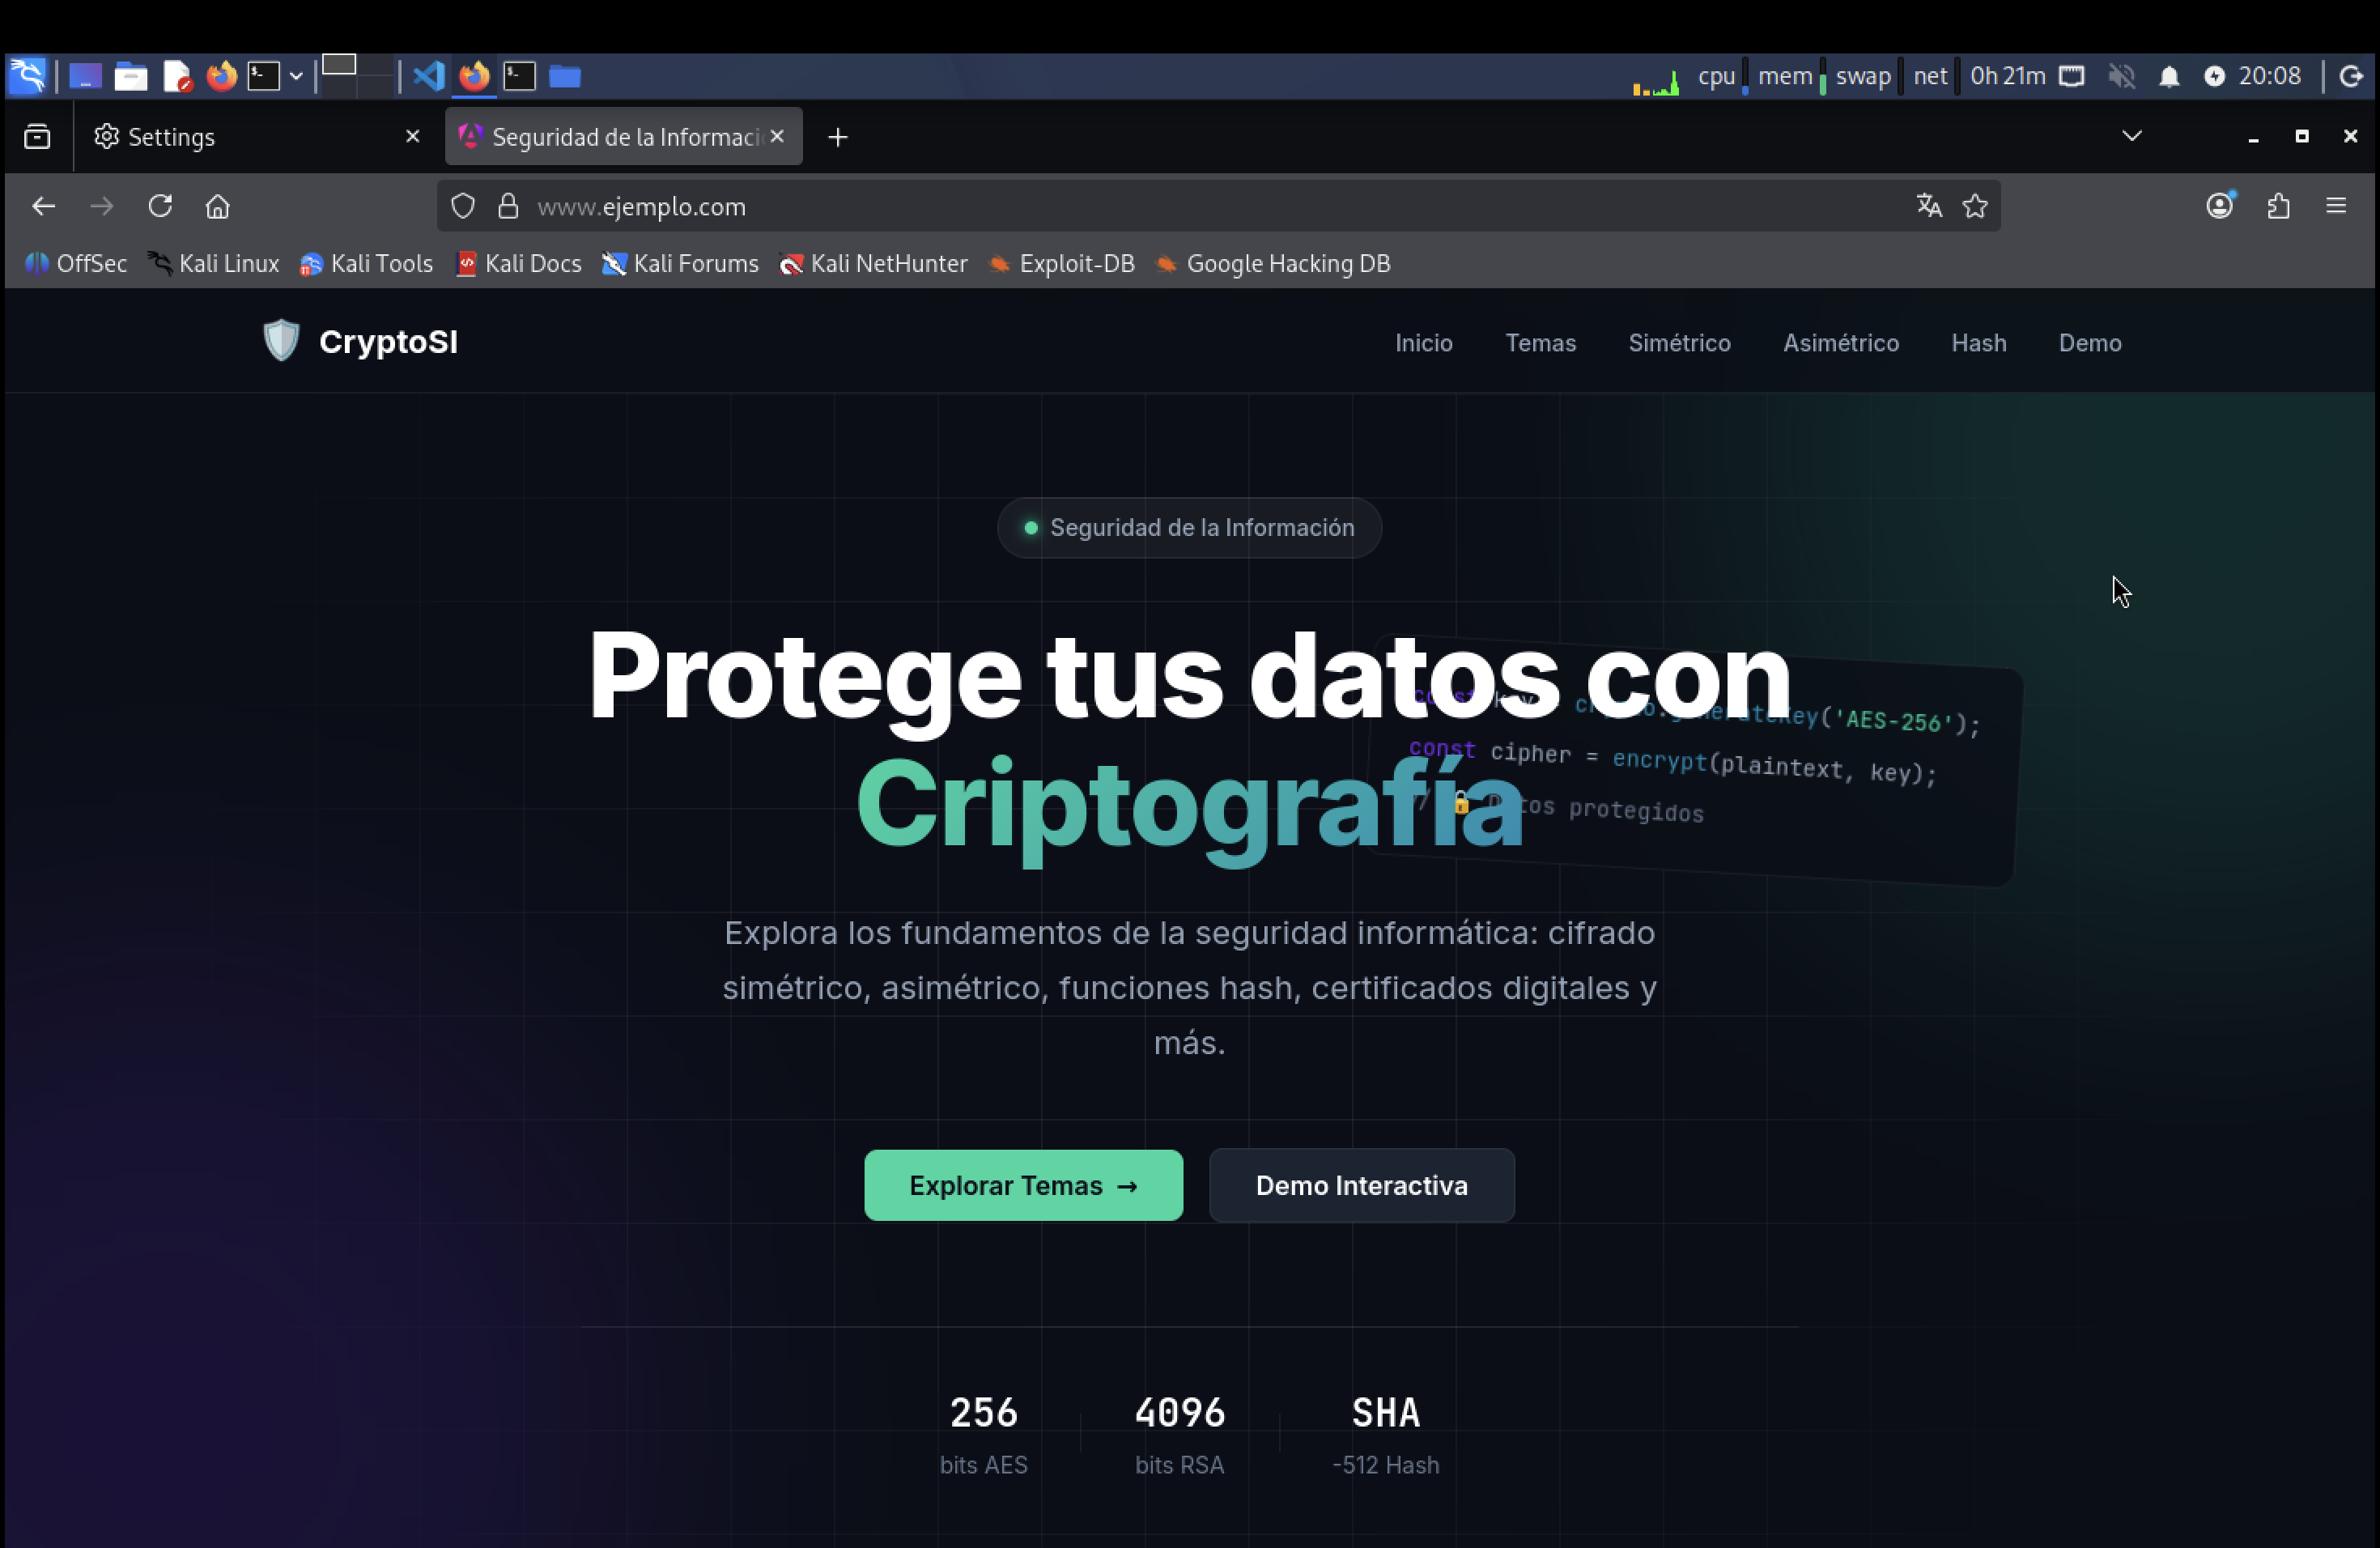
\includegraphics[width=0.8\textwidth]{Imagenes/20.png}
    
    \caption{Contenido de ejemplo.com.} 
    
    \label{fig:imagen_20} % Etiqueta para poder referenciarla más tarde
\end{figure}
\begin{figure}
    \centering     % Centra la imagen (buena práctica)

    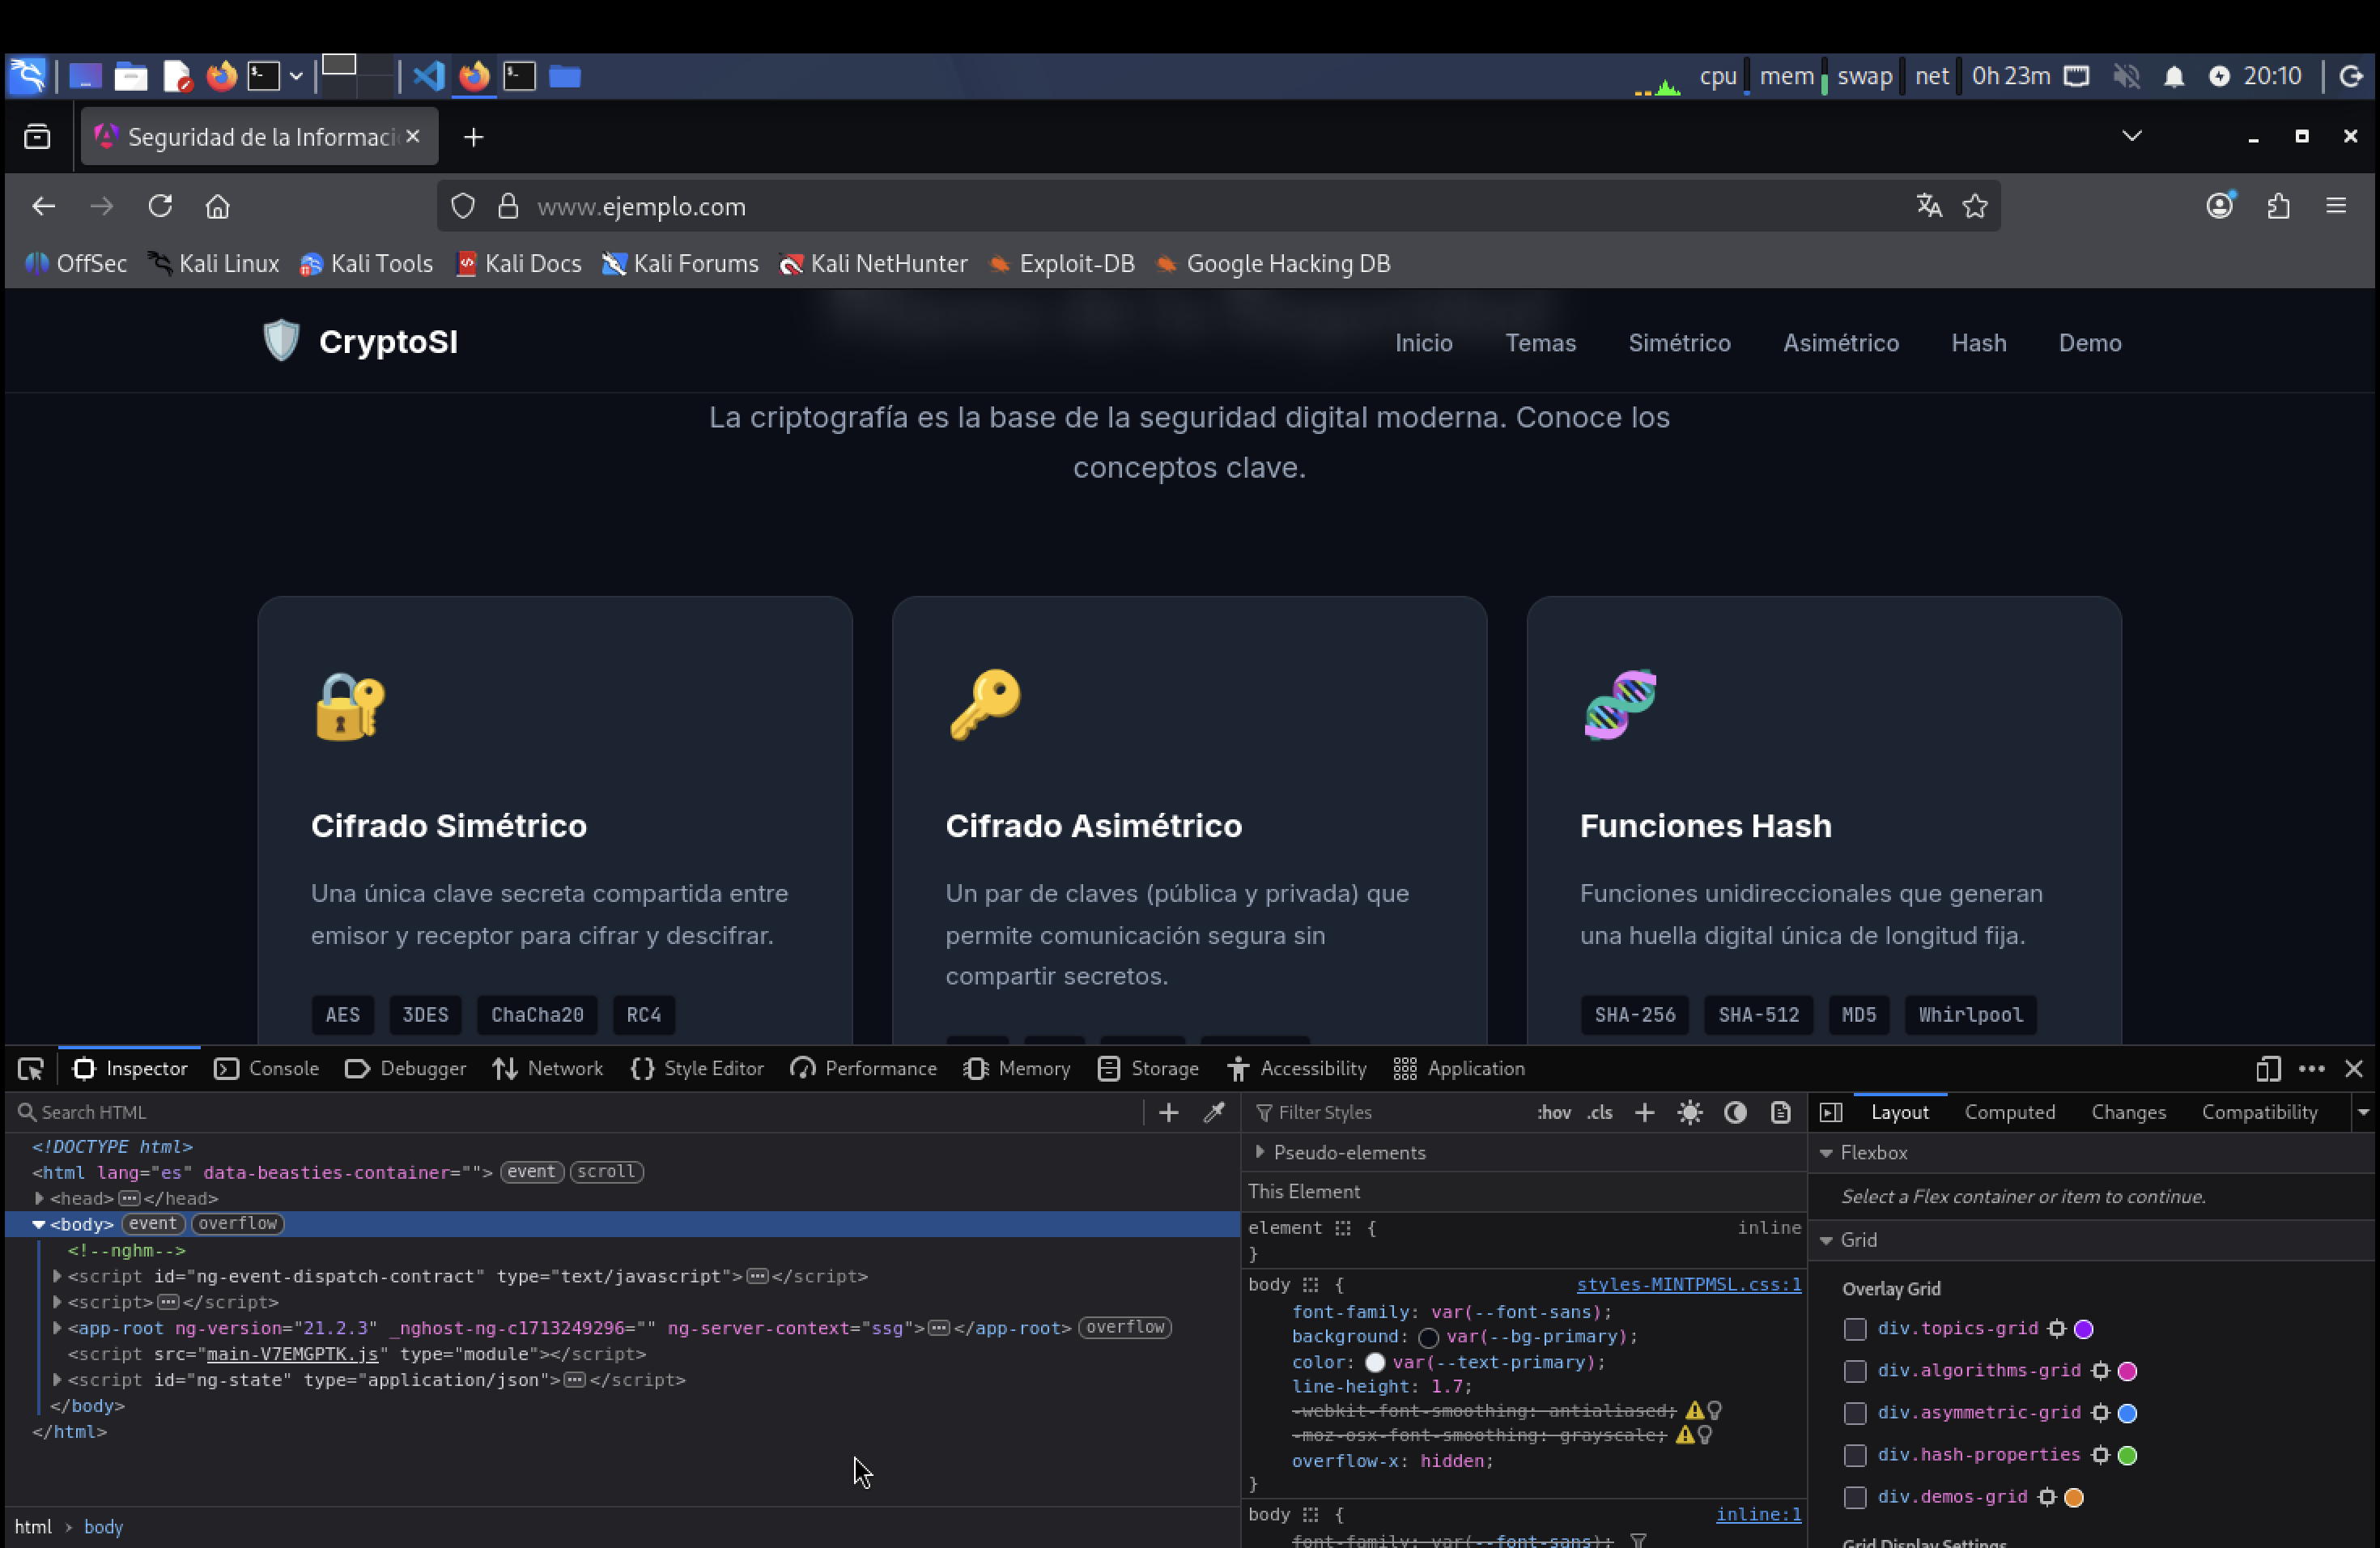
\includegraphics[width=0.8\textwidth]{Imagenes/21.png}
    
    \caption{Contenido de desarrollo de ejemplo.com.} 
    
    \label{fig:imagen_21} % Etiqueta para poder referenciarla más tarde
\end{figure}
\begin{figure}
    \centering     % Centra la imagen (buena práctica)

    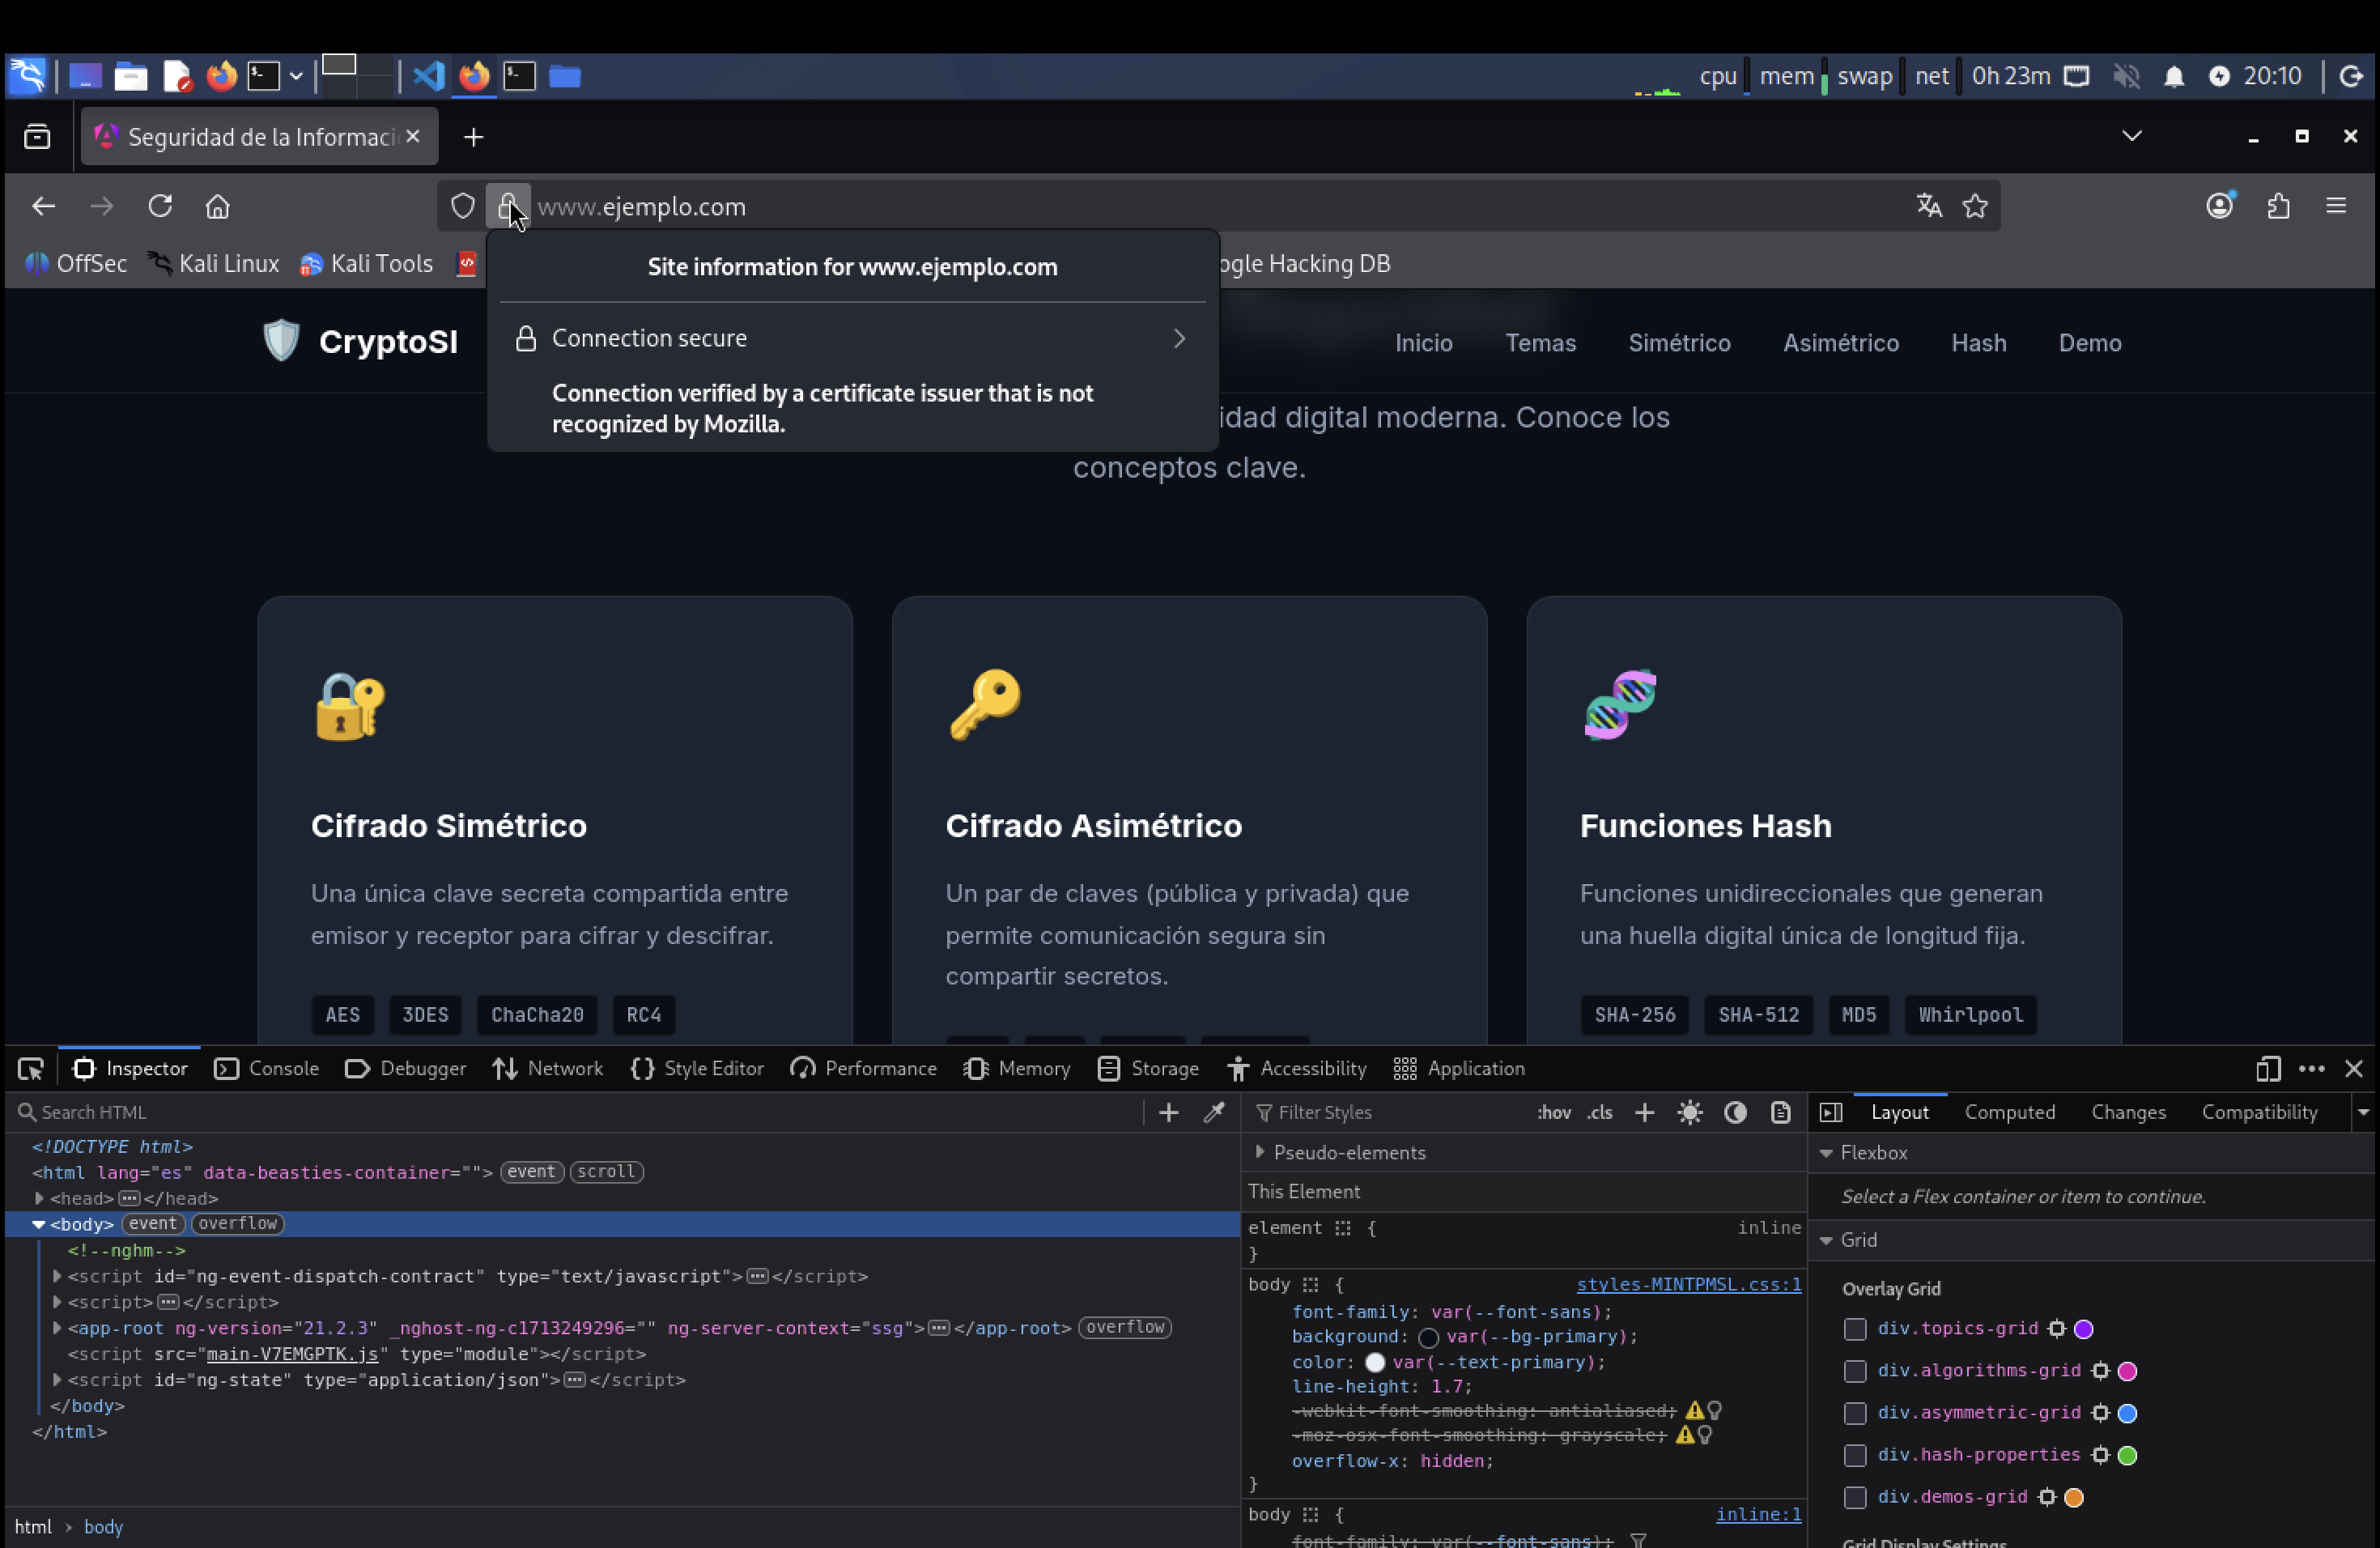
\includegraphics[width=0.8\textwidth]{Imagenes/22.png}
    
    \caption{Información de la conexión.} 
    
    \label{fig:imagen_22} % Etiqueta para poder referenciarla más tarde
\end{figure}
\begin{figure}
    \centering     % Centra la imagen (buena práctica)

    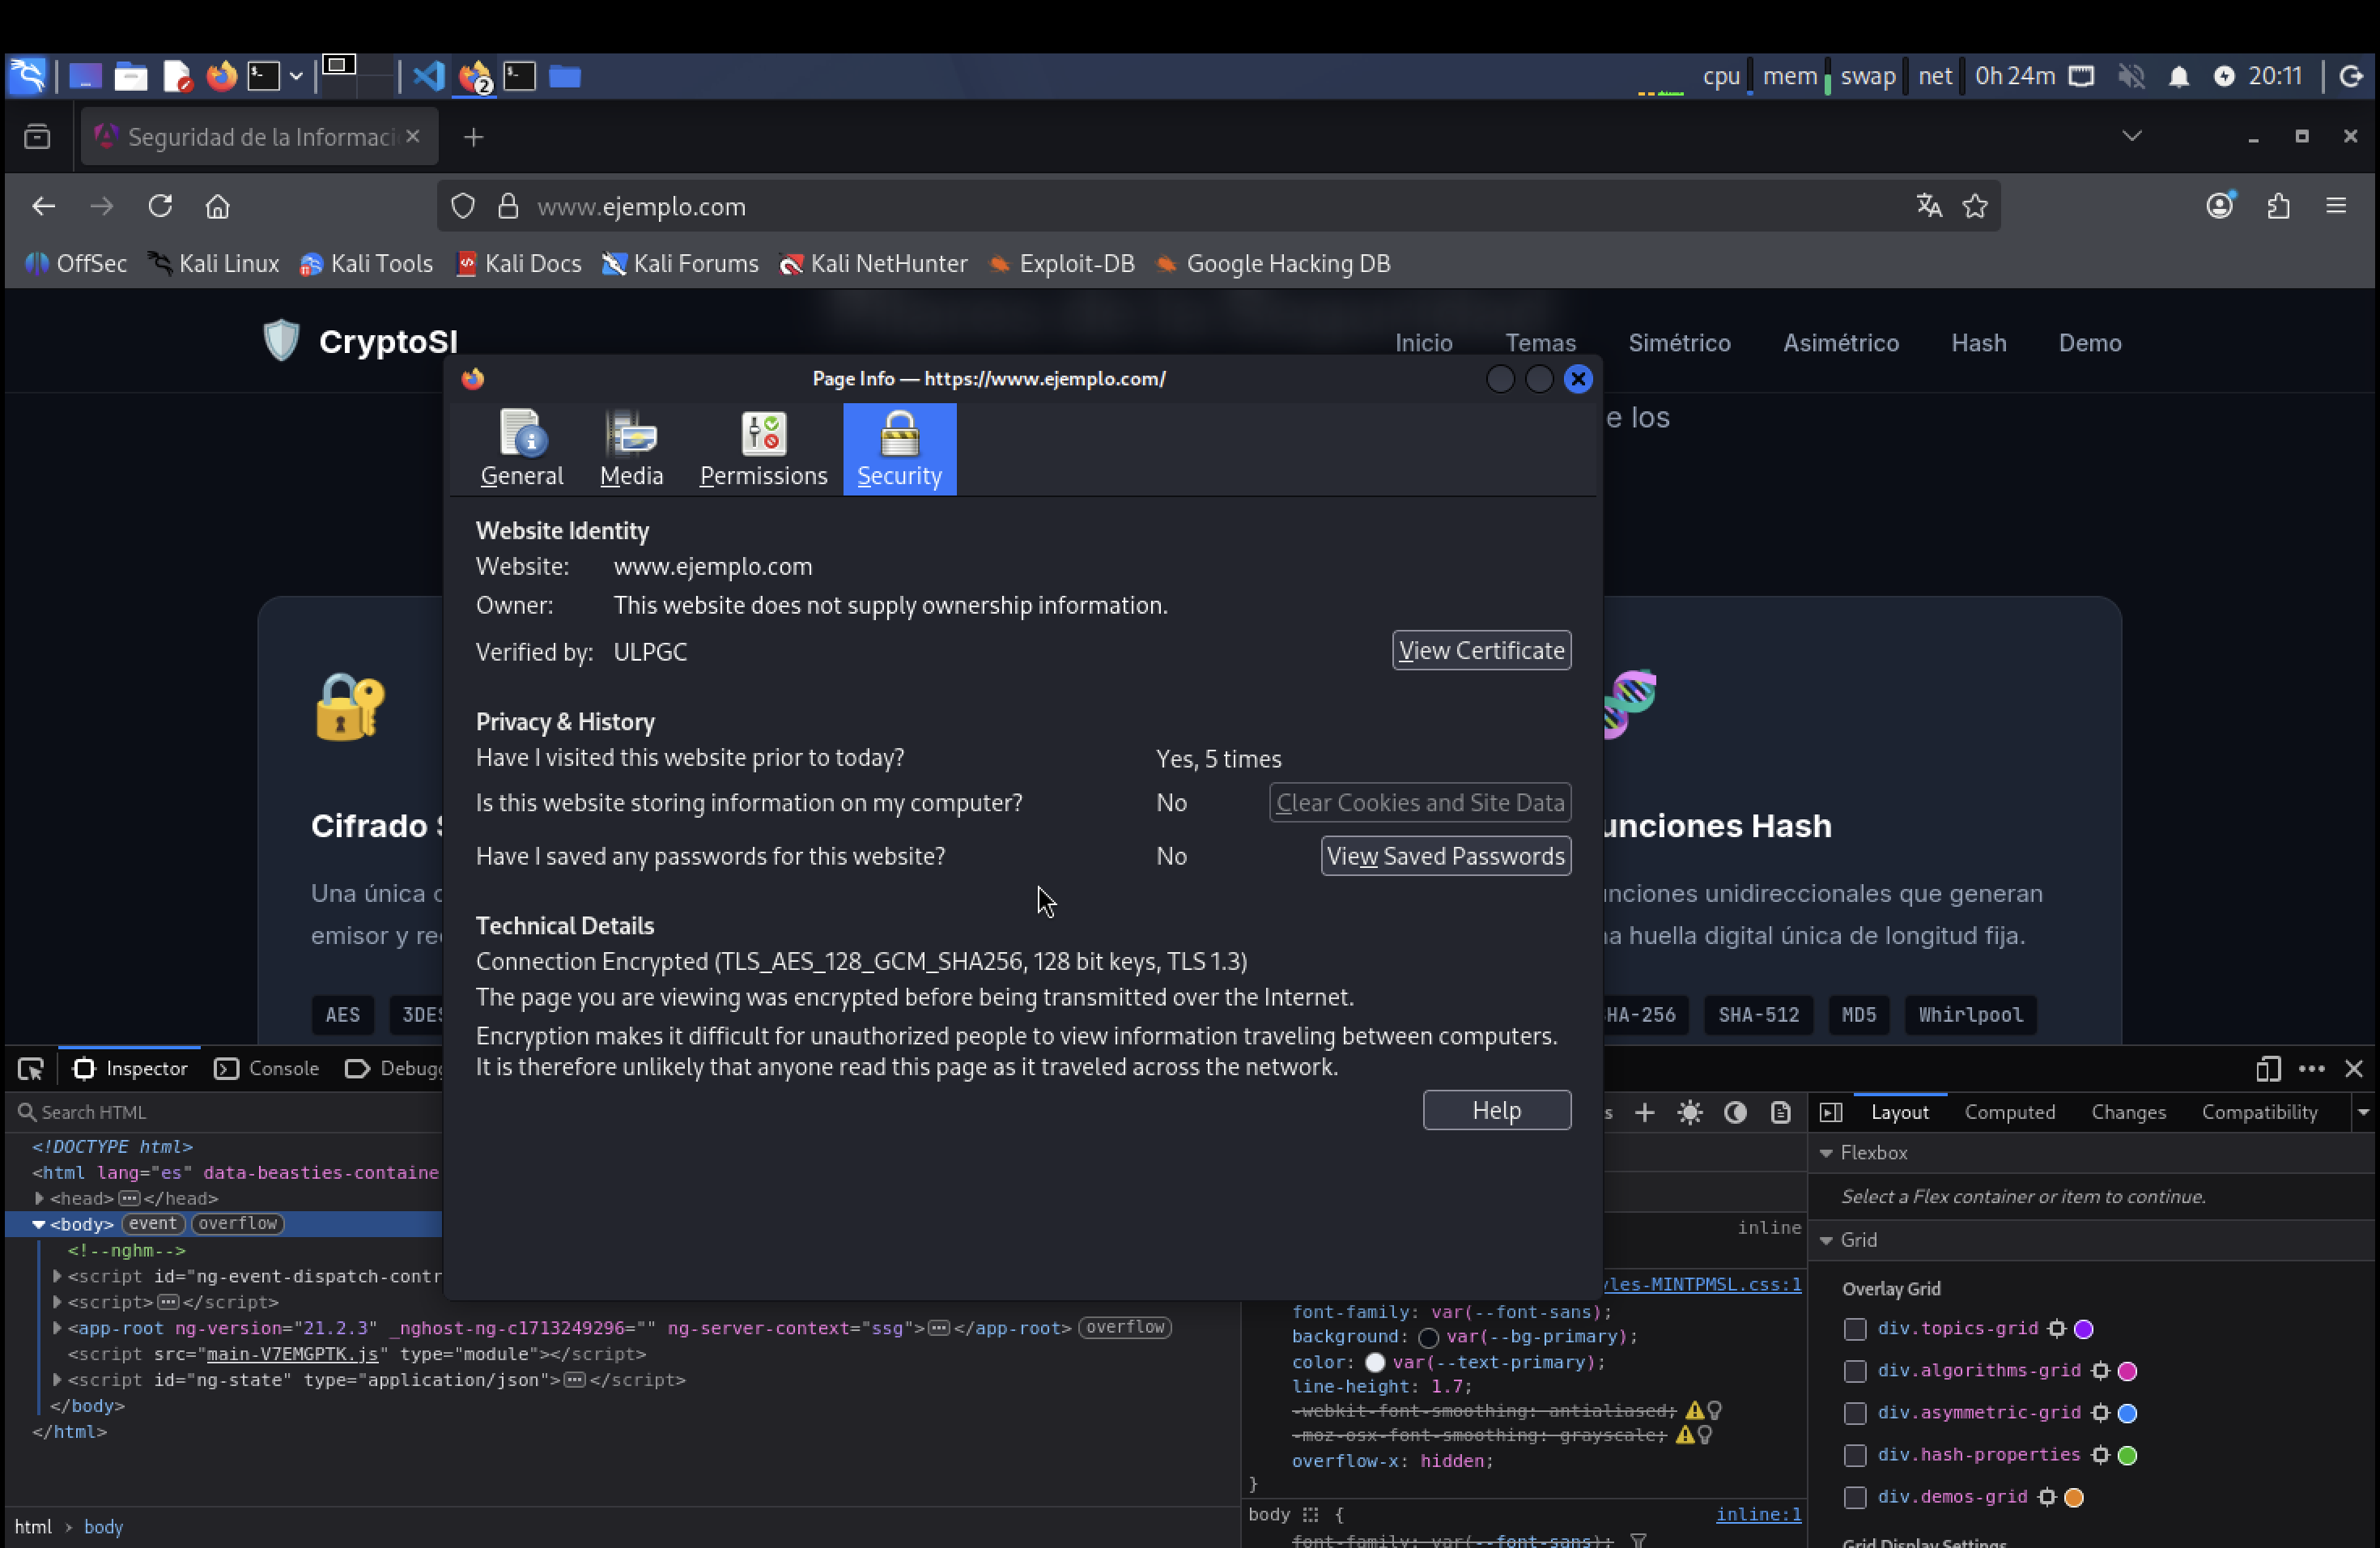
\includegraphics[width=0.8\textwidth]{Imagenes/23.png}
    
    \caption{Información avanzada de la conexión.} 
    
    \label{fig:imagen_23} % Etiqueta para poder referenciarla más tarde
\end{figure}